\section{Results}

Using the mesh of Figure \ref{fig:mesh}, that is, dividing the domain into 6 volumes (3 for each material), the resulting temperature profile is the one shown in Figure \ref{fig:6points}.
It should be noted that when evaluating the conductivity at the interface using the resistance method, the temperature values obtained are the same as the exact solution.
However, by assessing conductivity by linear variation, temperatures in material A are underestimated.
As the exact solution of the problem already has a linear behavior, and as the finite volume method is conservative, the discretization of the equations with the conductivity evaluated by the resistances method is equivalent to the analytical equations.
Therefore, using this method to calculate the thermal conductivity at the interface, the result will always be the exact one for this specific case, and without being influenced by the mesh size.

\begin{figure}[H]
    \centering
    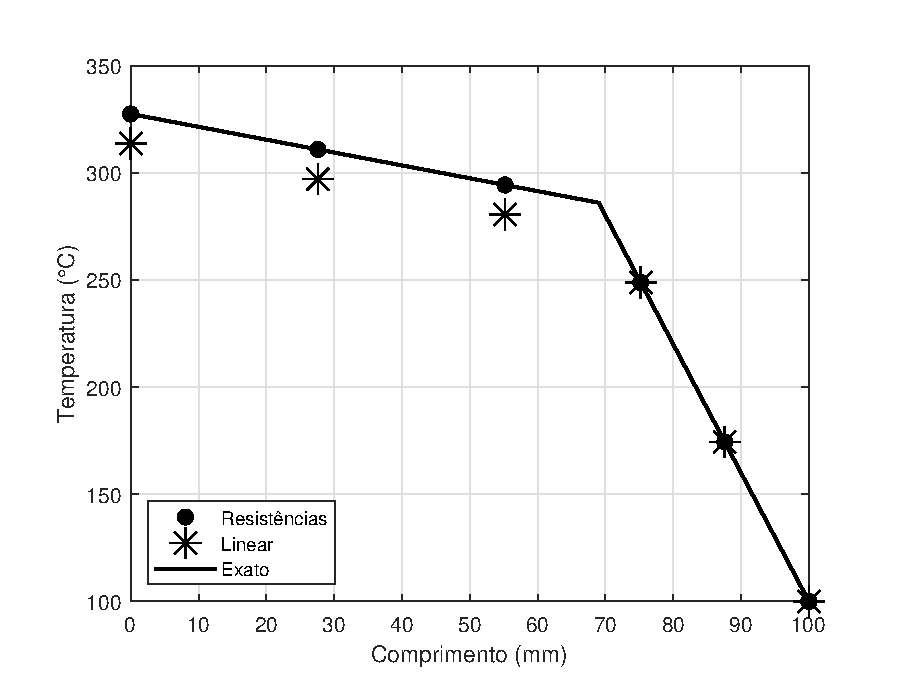
\includegraphics[scale=0.8]{6pontos.eps}
    \caption{Temperature profile with 6 control volumes in total.}
    \label{fig:6points}
\end{figure}

When increasing the number of control volumes to 20, with 10 volumes in each material, the temperature profile obtained is that of Figure \ref{fig:20points}.
It can be seen that the temperatures with the linear assessment of conductivity at the interface tend to approximate the exact result when refining the mesh.
This result is logical, since by decreasing the thickness of the control volumes, the calculation of the conductivity by linear variation becomes increasingly closer to the real value.
This behavior can be seen in Figure \ref{fig:error}, in which the absolute temperature error $T_1$ tends to be null, however, after a $N$ of about 40 volumes, the error decreases at a very fast rate in relation to the number of volumes.

\begin{figure}[H]
    \centering
    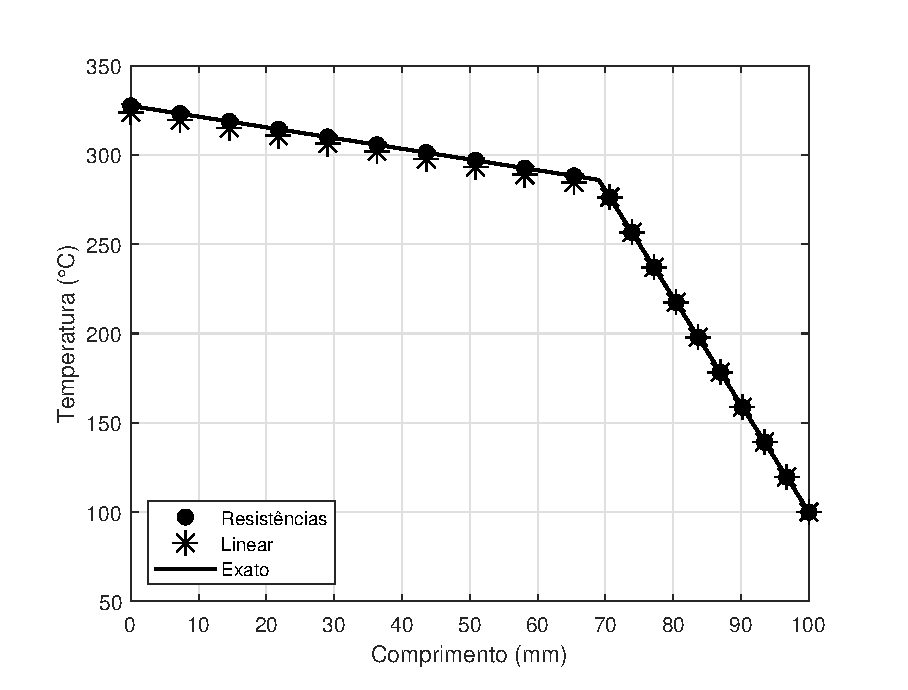
\includegraphics[scale=0.8]{20pontos.eps}
    \caption{Temperature profile with 20 control volumes in total.}
    \label{fig:20points}
\end{figure}

\begin{figure}[H]
    \centering
    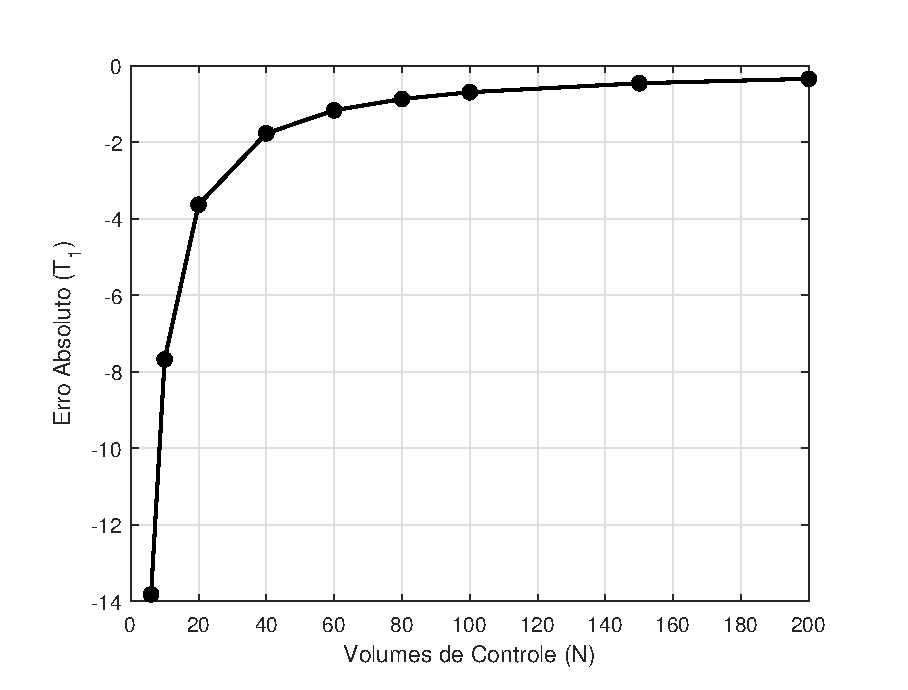
\includegraphics[scale=0.8]{erro.eps}
    \caption{Absolute temperature error on the left border when varying the number of control volumes and using the linear variation of conductivity at the interface.}
    \label{fig:error}
\end{figure}